
\chapter{Introducción}
\label{chap:intro} 
En este capítulo se introducen los conceptos básicos en los que se apoya este proyecto. Se explican y se ponen en contexto las tecnologías web y el estado actual de la robótica y su expansión hasta llegar al punto en el que se encuentra, haciendo especial mención a la robótica educativa en la que se centra el proyecto.
   
\section{Tecnologías web}
\label{sec:web}
Las tecnologías web han ido evolucionando a los largo de la historia, pero todas se basan en un modelo cliente-servidor. Para lograr la comunicación entre cliente y servidor, se necesita un navegador por parte del cliente y un servidor web capaz de atender las solicitudes. El protocolo que es utilizado para esta comunicación se llama \textit{HTTP}.

\subsection{HTTP}
\label{subsec:http}
\textit{HTTP} (\textit{HiperText Transfer Protocol}) es el protocolo de nivel de aplicación utilizado para transferir recursos hipermedia entre ordenadores y sigue el esquema petición-respuesta entre cliente y servidor (Figura \ref{fig:http}). En esta comunicación el cliente abre una conexión \textit{TCP} con el servidor y envía un mensaje de petición \textit{HTTP} y, por parte del servidor, responde al cliente con un mensaje \textit{HTTP} y cierra la conexión \textit{TCP}. 
El protocolo \textit{HTTP} no mantiene estado. Es decir, el servidor trata cada petición de manera aislada y no almacena información sobre peticiones realizadas por un mismo cliente. 
Las peticiones están definidas por el protocolo y tienen métodos concretos: 
\begin{itemize}
    \item GET: Solicita un recurso al servidor especificando su \textit{URL}.
    \item HEAD: Método similar a GET con la diferencia de que únicamente solicita las cabeceras y no descarga el recurso completo.
    \item POST: Envía datos al servidor, normalmente un recurso específico que provoca un cambio de estado. 
    \item PUT: Actualiza información sobre un recurso del servidor. 
    \item DELETE: Elimina en el servidor un recurso.
\end{itemize}

Aunque estos son los principales métodos, el protocolo tiene flexibilidad para ir añadiendo nuevos e incorporar funcionalidad. El número de métodos se han ido aumentando con las nuevas versiones. 
\begin{figure}[h]
\centering
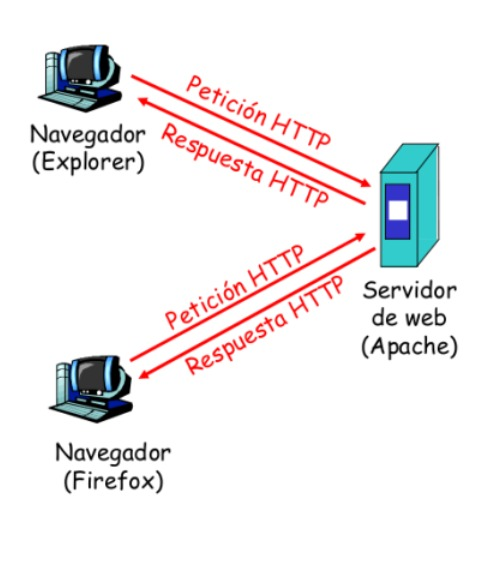
\includegraphics[scale=0.4]{img/http.jpeg}
\caption{Comunicación cliente-servidor en HTTP} \label{fig:http}
\end{figure}

Aunque la versión actual del protocolo data del 2 de abril de 2019 (\textit{HTTP/2.4.38}), es en 1991 cuando se lanza la primera versión y, en el mismo año, se publica un estándar para la publicación de páginas web mediante un lenguaje de marcas de hipertexto (\textit{HTML}), que se explicará en el siguiente apartado. 

\subsection{Tecnologías en cliente}
\label{subsec:tecclient}
Es la parte encargada de dar forma a la interfaz de usuario y de establecer la comunicación con el servidor. Una pieza importante del cliente es el navegador, ya que es el encargado de leer e interpretar la información recibida. Las más utilizadas son: 
\begin{itemize}
    \item \textit{HTML}: es el estándar más utilizado para el desarrollo de páginas web. Actualmente los navegadores usan la versión \textit{HTML5}. Este lenguaje indica la estructura de una página web, para editar el estilo y presentación visual hay que hacer uso de otros elementos como \textit{CSS}.
    \item \textit{CSS}: \textit{Cascading Style Sheets} es un lenguaje de diseño gráfico para definir y crear la presentación de un documento escrito en un lenguaje de marcado. De esta forma, se permite separar información y datos (en los documentos \textit{HTML}) y todo lo relativo al diseño y presentación (en documentos \textit{CSS}). Actualmente los navegadores usan la versión \textit{CSS3}.
    \item \textit{JavaScript}: para programar la lógica, dinamismo e interacción con el usuario es el lenguaje más común y extendido en el desarrollo de páginas. Debido a su importancia en el proyecto, se explicará más a fondo en próximos capítulos. 
\end{itemize}

\subsection{Tecnologías en servidor}
\label{subsec:tecserver}
Son las encargadas de dar forma al servidor web de manera que permite el acceso a herramientas como base de datos, conexiones de red o recursos compartidos. O, dicho de otra forma, se ocupan de realizar las tareas necesarias para hacer posible crear una aplicación que visualizará el cliente. Las más utilizadas son: 
\begin{itemize}
    \item \textit{Node.js}: es una forma de ejecutar \textit{JavaScript} en el servidor. Proporciona un entorno de ejecución del lado del servidor que compila y ejecuta a gran velocidad.  Esto es debido a que compila en código máquina nativo en lugar de interpretarlo o ejecutarlo.   
    \item \textit{Django}: entorno web de alto nivel programado en \textit{python} diseñado para realizar aplicaciones de cualquier complejidad. Es seguro, rápido y escalable. Además, incluye una interfaz para acceder a bases de datos lo que facilita las consultas al no tener que manejar \textit{SQL} y realizarlas con filtros de \textit{Python}.
    \item \textit{Spring}: herramienta que tiene la finalidad de simplificar el desarrollo de aplicaciones ya que facilita la configuración de la aplicación y el despliegue en servidor. De esta manera, \textit{Spring} está pensado para aplicaciones web, servicios \textit{REST}, análisis de datos o integración de sistemas. 
\end{itemize}

\section{Robótica}
\label{sec:robotica}
La robótica es una rama tecnológica encargada del diseño y construcción de aparatos que realizan operaciones y trabajos en sustitución de la mano de obra humana. 

Un robot es un sistema autónomo programable capaz de realizar tareas de ayuda al ser humano y con aplicaciones en campos diversos como medicina, hogar, fábricas, etc. 

Los robots se componen de sensores, controladores y actuadores.
\begin{itemize}
    \item \textbf{Sensores}: son los encargados de recoger información del entorno. En este grupo se encuentran láser, cámaras, ultrasonidos u odómetros. Estos dispositivos equivalen a los sentidos humanos. 
    \item \textbf{Controladores}: analizan los datos recogidos por los sensores y elaboran una respuesta que va a ser enviada a los actuadores. En los seres humanos equivale al cerebro. 
    \item \textbf{Actuadores}: se encargan de transformar energía eléctrica, hidráulica o neumática en mecánica. Son los interactúan con el entorno y equivalen a los músculos humanos. 
\end{itemize}

\subsection{Historia}
La palabra robot fue empleada por primera vez en 1920 por Karel Capek, un escritor checo que realiza una obra de teatro en la que un hombre fabrica un robot. 

Años más tarde, en 1950, Isaac Asimov publica un libro llamado \textit{Yo, Robot} en el que acuña la palabra robótica definiendo a la ciencia que estudia a los robots. En el también se incluyen tres leyes de la robótica:
\begin{itemize}
    \item Un robot no hará daño a un ser humano ni permitirá que un ser humano sufra ningún tipo daño.
    \item Un robot debe cumplir las órdenes recibidas por un ser humano, salvo las que entren en conflicto con la primera ley.
    \item Un robot debe proteger su propia existencia mientras que no entre en conflicto con ninguna de las leyes anteriores. 
\end{itemize}{}

Es a finales de la década de los 50 cuando la robótica sufre el mayor impulso al crearse el primer robot comercial en 1956 y, años más tarde, en 1961, se instala el primer robot industrial (Figura \ref{fig:unimate}).  

\begin{figure}[H]
\centering
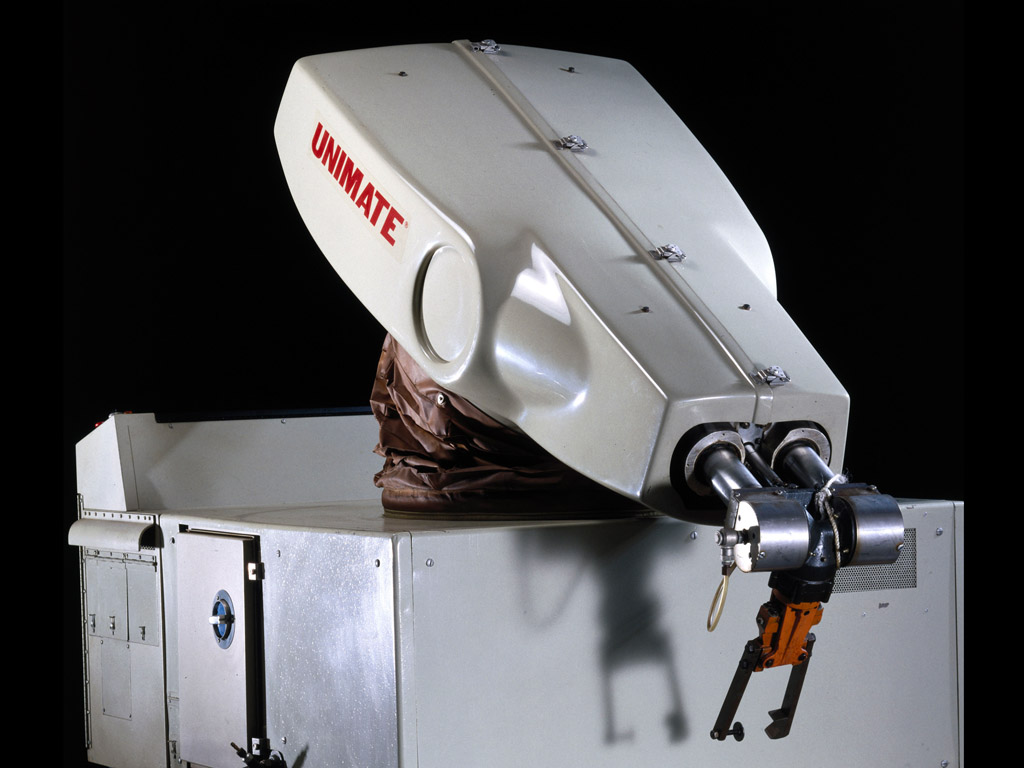
\includegraphics[width=0.6\textwidth]{img/unimate.jpg}
\caption{Unimate, primer robot industrial} \label{fig:unimate}
\end{figure}

En los años 70 se crea el primer robot autónomo, \textit{Shakey}  (Figura \ref{fig:shakey}). Fue el primero que incorporaba inteligencia artificial y disponía de control de motores y sensores. \textit{Shakey} era capaz de recoger toda la información de su entorno, crear un mapa y diseñar el camino más corto desde su ubicación al destino. 

\begin{figure}[H]
\centering
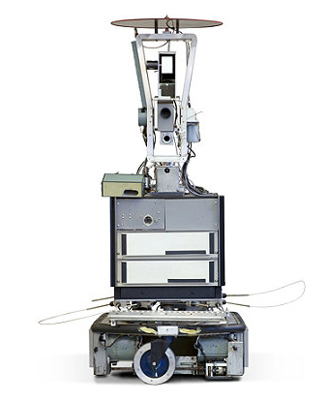
\includegraphics[width=0.5\textwidth]{img/shakey.jpg}
\caption{Shakey, primer robot autónomo} \label{fig:shakey}
\end{figure}

En 2000 la compañía Honda lanza el robot \textit{Asimo} (Figura \ref{fig:asimo}), un robot humanoide capaz de detectar múltiples objetos, reconocer caras e interpretar comandos de voz o gestos.\textit{Asimo} fue creado con el objetivo de, algún día, ofrecer asistencia a personas con necesidades especiales. 

\begin{figure}[H]
\centering
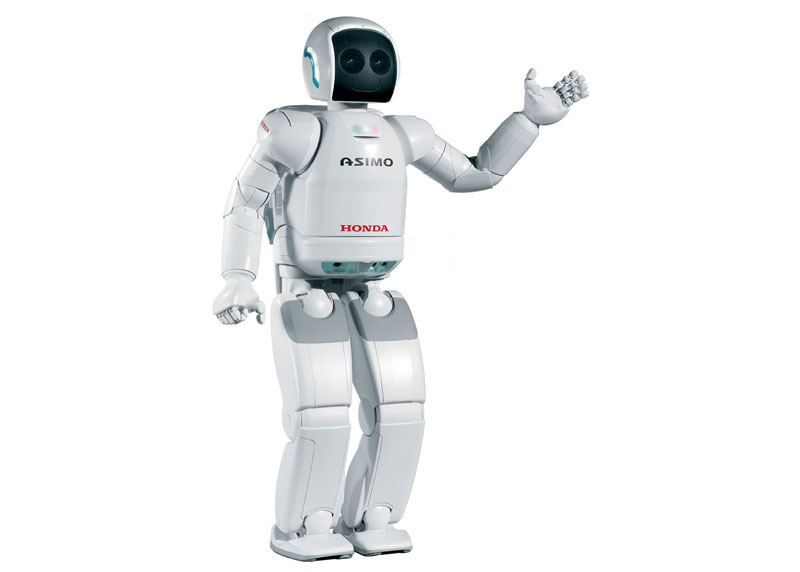
\includegraphics[width=0.5\textwidth]{img/asimo-honda.jpg}
\caption{Asimo, primer robot humanoide} \label{fig:asimo}
\end{figure}

Es en 2011 cuando la robótica alcanza uno de sus mayores hitos gracias al robot explorador \textit{Curiosity} (Figura \ref{fig:curiosity}). Este robot llego a Marte en 2012 y su cometido fue investigar el planeta para determinar si existió vida en Marte, caracterizar su clima y geología y preparar el entorno para su exploración humana. 

\begin{figure}[H]
\centering
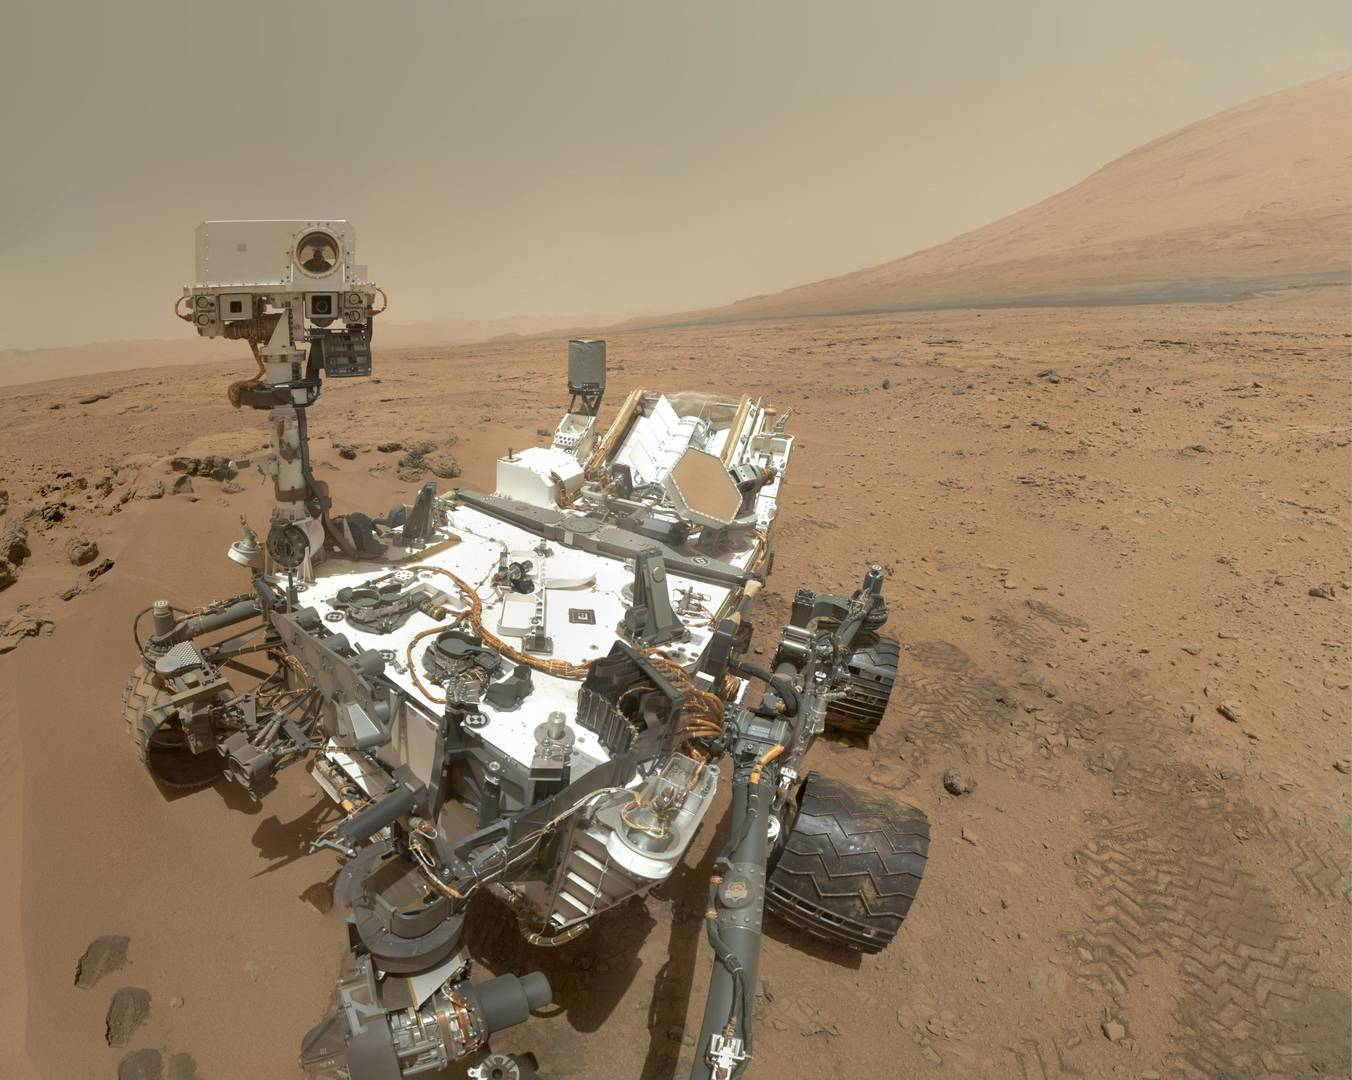
\includegraphics[width=0.6\textwidth]{img/curiosity.jpg}
\caption{Autorretrato del Curiosity en Marte} \label{fig:curiosity}
\end{figure}


Hoy en día no solo se ven robots en entornos industriales, si no que aparecen cada vez más en entornos domésticos, educativos o automovilístico.

\subsection{Tipos de robots}
\label{subsec:tiposRobots}
Los ámbitos en los que se encuentra la robótica son diversos. Los tipos en los que podemos dividir los tipos de robots son: 
\begin{itemize}
    \item \textbf{Industriales}: son los utilizados para mover materiales pesados, herramientas y realizar una serie de tareas en ambientes de producción y manufactura. Este tipo de robots permiten realizar trabajos peligrosos y repetitivos sin cometer errores, por lo que están revolucionando la industria y cada vez es más común verlos en las fábricas.   
    \item \textbf{Militares}: robots autónomos o controlados de manera remota diseñados para transporte, búsqueda, rescate o ataque. Destacan drones usados para espionaje o recolección de datos e imágenes. 
    Existen muchas funciones que son realizadas por este tipo de robots, es común la supervisión humana para controlar que el criterio del robot sea correcto frente posibles amenazas. 
    \item \textbf{Espaciales}: son aquellos que se utilizan en exploraciones de terrenos y ambientes de otros planetas o como apoyo al trabajo de los astronautas. 
    \item \textbf{Medicina}: involucra varios ámbitos sanitarios y tiene grandes ventajas. Desde sistemas de desinfección eficientes (como el robot \textit{Xenex}\footnote{\url{https://www.xenex.com}}), herramienta para desinfectar instalaciones médicas) hasta robots que pueden reemplazar o ayudar a cirujanos por su precisión y eficiencia (robot \textit{Da Vinci}\footnote{\url{https://www.intuitive.com}}, que permite tener un campo de visión magnificado e instrumental médico mejorado). 
    \item \textbf{Robots de servicio}: este tipo de robots mejoran la productividad en casi cualquier tarea dando la posibilidad de automatizar cualquier tipo de tarea que requiera eficiencia y rapidez. Pueden operar de forma autónoma y pueden formar parte robots desde aspiradores robóticos (como el robot   \textit{Roomba}\footnote{\url{https://www.irobot.es}}) hasta sistemas domóticos (como el altavoz desarrollado por \textit{Google}, \textit{Google Home}\footnote{\url{https://store.google.com/es/product/google_home}}).
    \item \textbf{Entretenimiento}: son algunos de los robots más sofisticados ya que requieren interactuar con personas. Se pueden encontrar desde juguetes hasta robots que ayuden a la enseñanza. En este último tipo se entrará más en detalle por ser un pilar fundamental del proyecto.
\end{itemize}
\section{Robótica educativa}
\label{sec:educativa}


La robótica con fines educativos está empezando a adquirir importancia en la enseñanza porque su aprendizaje está disponible para estudiantes de cualquier nivel. Este método de enseñanza intenta despertar el interés de los estudiantes cambiando asignaturas tradicionales y convirtiéndolas en atractivas e integradoras. \newline

Es importante empezar poco a poco y para preparar a los más jóvenes y tener nociones básicas de la robótica por la importancia que esta adquiriendo esta disciplina pues ya se empiezan a implantar robots en la mayor parte de los sectores laborales. \newline

La enseñanza en centros escolares se realiza en gran parte mediante plataformas como la creada por LEGO o placas Arduino que simplifican el aprendizaje y resulta motivadora para el alumno porque obtiene resultados vistosos y se le puede dar una aplicación real. \newline



La capacidad de programar es una parte importante en la sociedad actual ya que, con esta habilidad, se aprenden estrategias para resolver problemas, diseñar proyectos y comunicar ideas. Es por eso que se intenta inculcar programación desde cortas edades y se realiza mediante lenguajes de programación visual. Se trata de lenguajes de programación potentes que abstraen al alumno de la complejidad que implica la sintaxis, son muy intuitivos y aportan un entorno visual haciendo que el software sea bien aceptado por estudiantes de corta edad. Estos lenguajes permiten a los usuarios programar manipulando elementos gráficos del en lugar de hacerlo textualmente. Los lenguajes de programación visual más importantes son: 

\begin{itemize}
    \item \textit{Scratch}: proyecto liderado por el \textit{MIT} y es utilizado por estudiantes y docentes para programar animaciones, juegos e interacciones fácilmente gracias a su interfaz visual. Se trata de un lenguaje donde los programas se construyen ensamblando bloques gráficos y cada bloque es el equivalente a una función o método de cualquier lenguaje de programación. Actualmente está en su versión \textit{Scratch 3.0} y en la figura \ref{fig:scratch} se puede ver un ejemplo de su interfaz gráfica. 
    \begin{figure}[H]
    \centering
    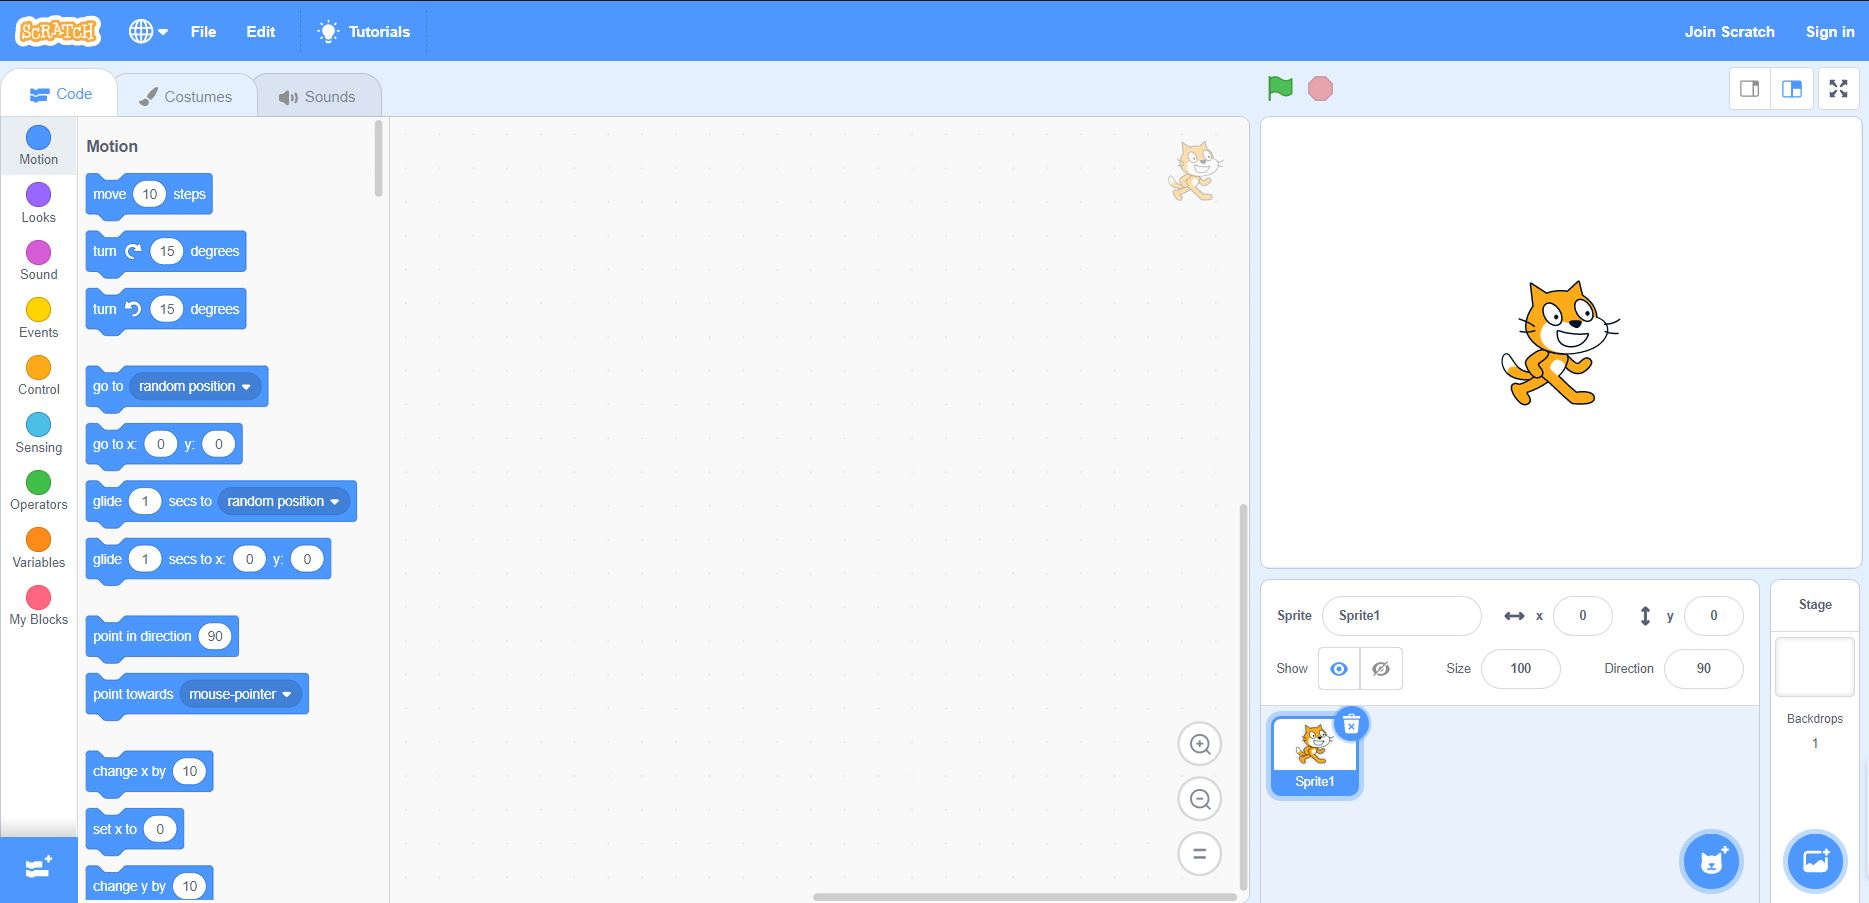
\includegraphics[width=1\textwidth]{img/scratch.jpg}
    \caption{Interfaz gráfica de Scratch} \label{fig:scratch}
    \end{figure}
    
    \item \textit{Blockly}: proyecto de \textit{Google} diseñado para el lenguaje de programación \textit{JavaScript} pensado para crear lenguajes de programación visual. Se ejecuta en un navegador web y visualmente recuerda a \textit{Scratch}. Hablaremos en capítulos siguientes más en profundidad. 
    
    \item \textit{LEGO}: dispone de una amplia gama de robots programables y cada uno de ellos tiene un sistema de programación bajo interfaz gráfica. En las figuras \ref{fig:lego1} y \ref{fig:lego2} se pueden ver dos ejemplos de distintos software para distintos robots.  
    
    
    \begin{figure}[h]
    \centering
        \begin{subfigure}{0.45\textwidth}
           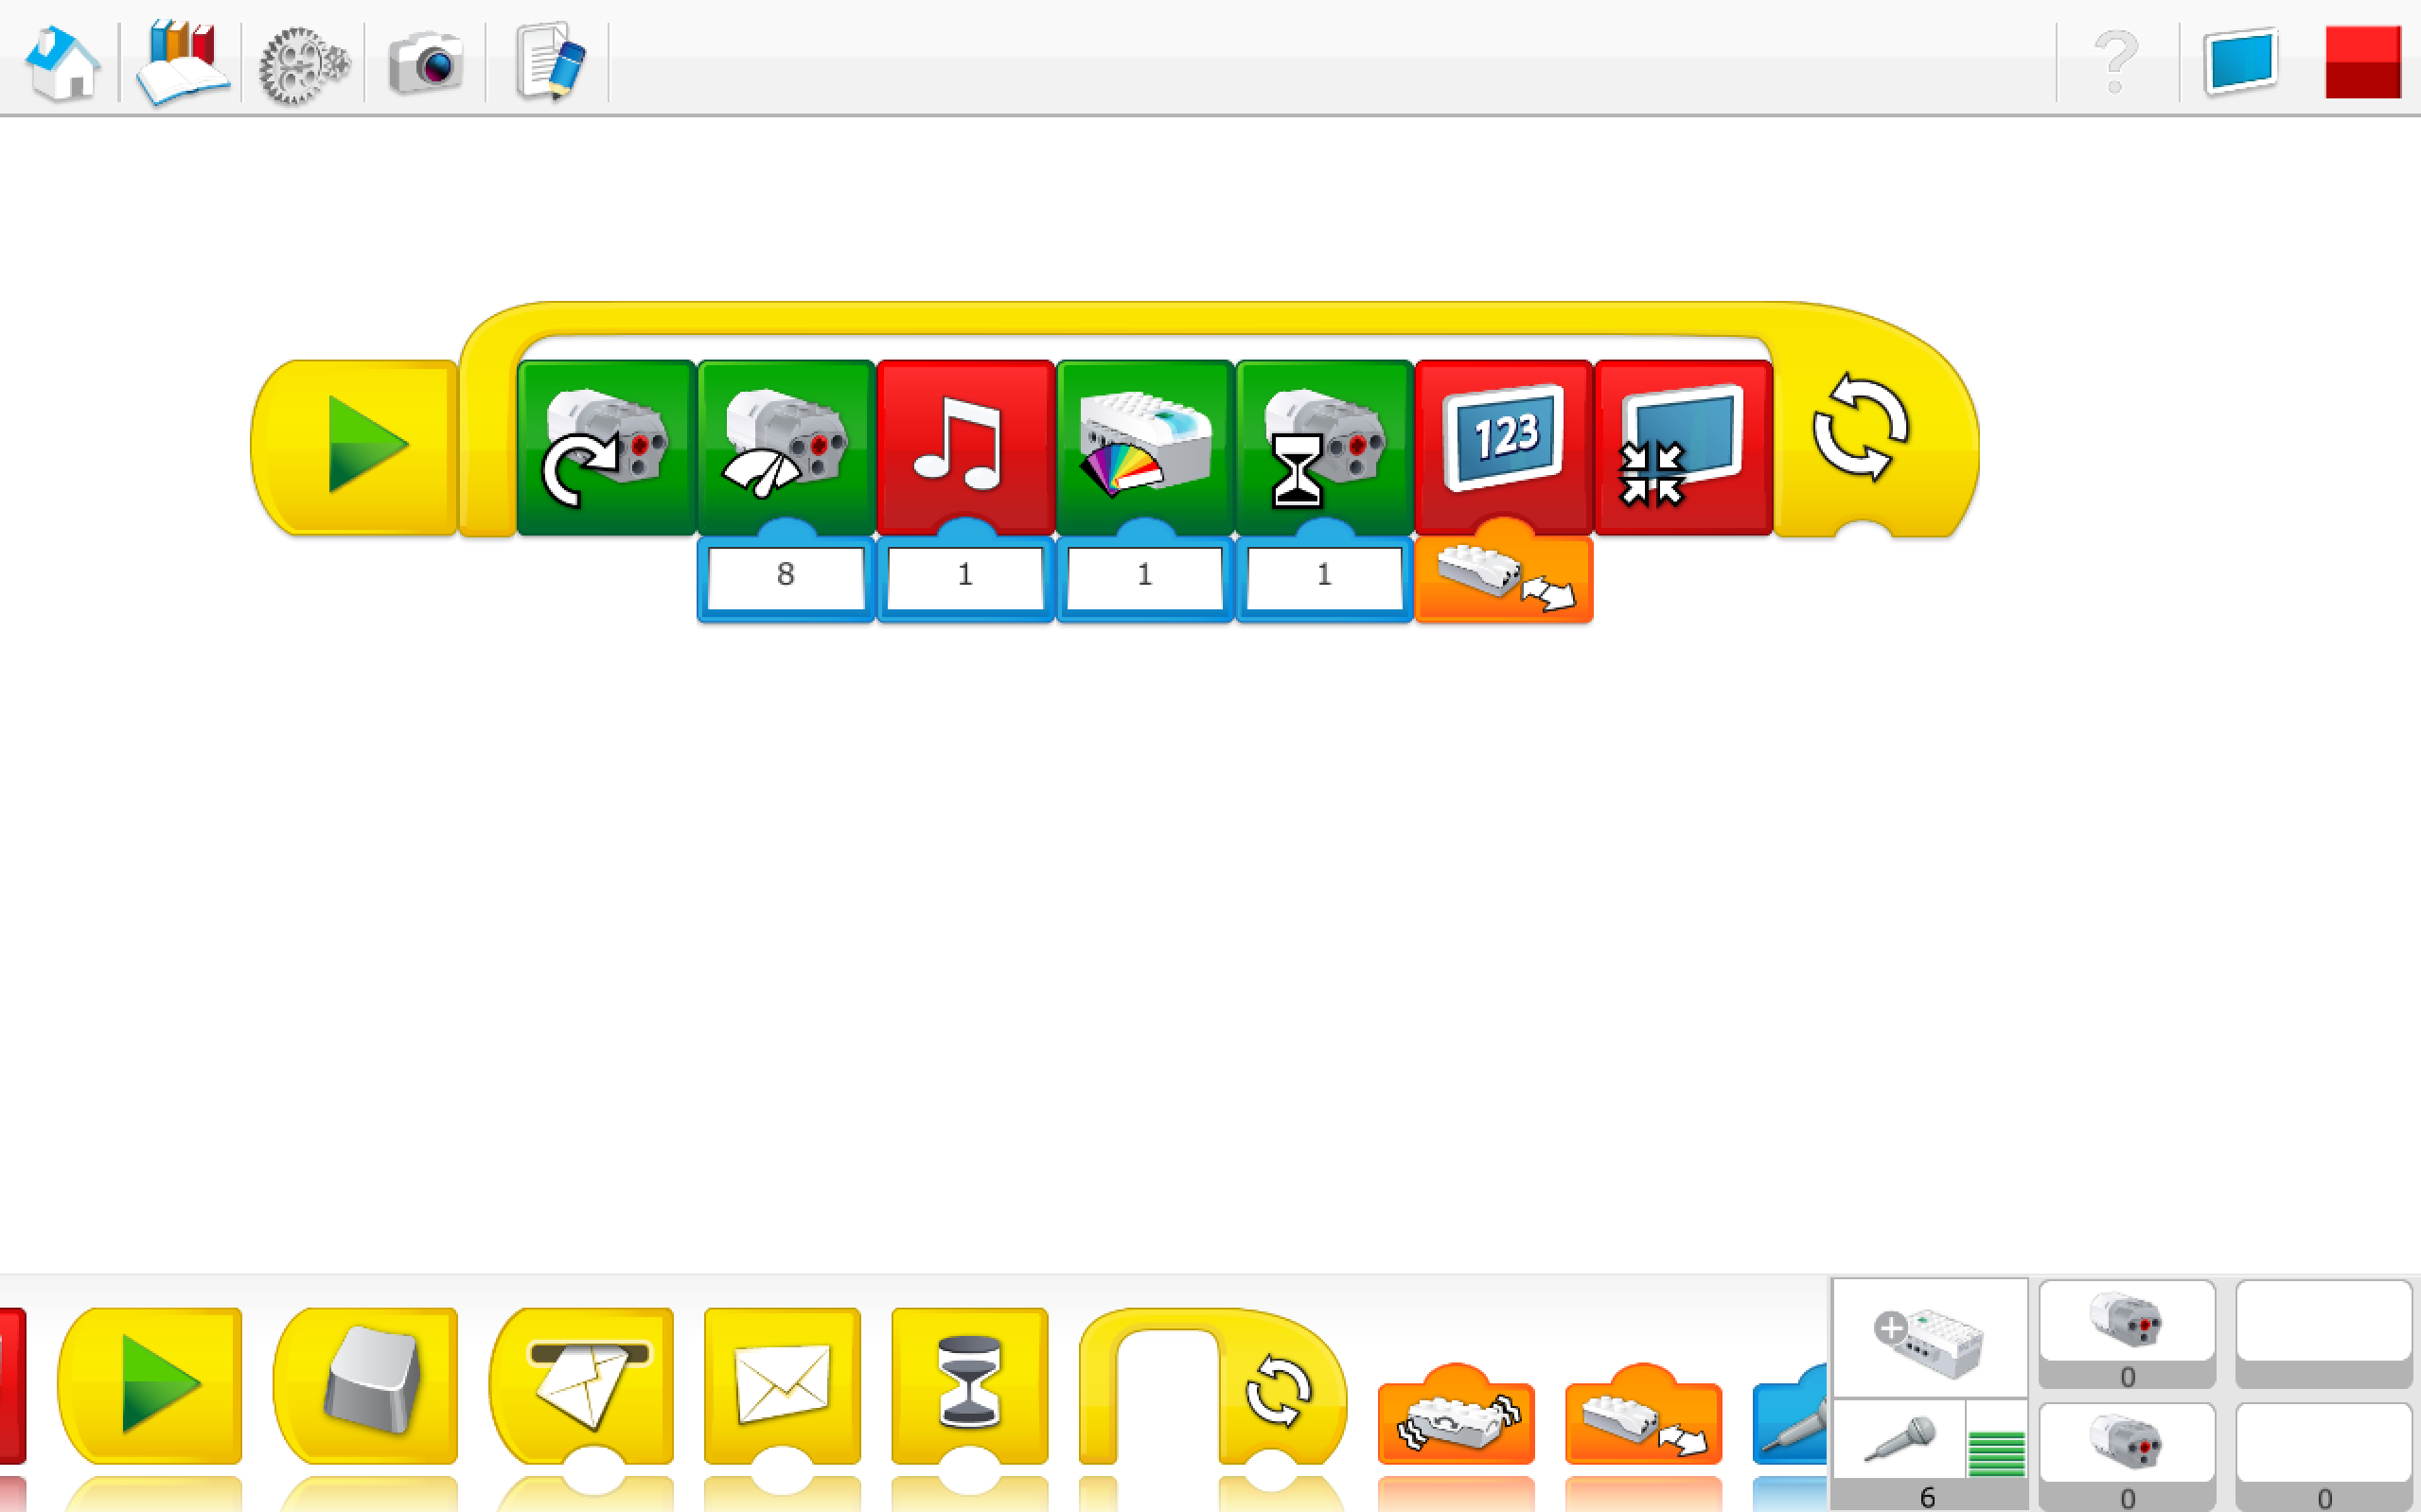
\includegraphics[width=\textwidth]{img/lego1.png}
           \caption{Interfaz gráfica de LEGO WeDo 2.0} 
            \label{fig:lego1}
        \end{subfigure}
        \begin{subfigure}{0.45\textwidth}
            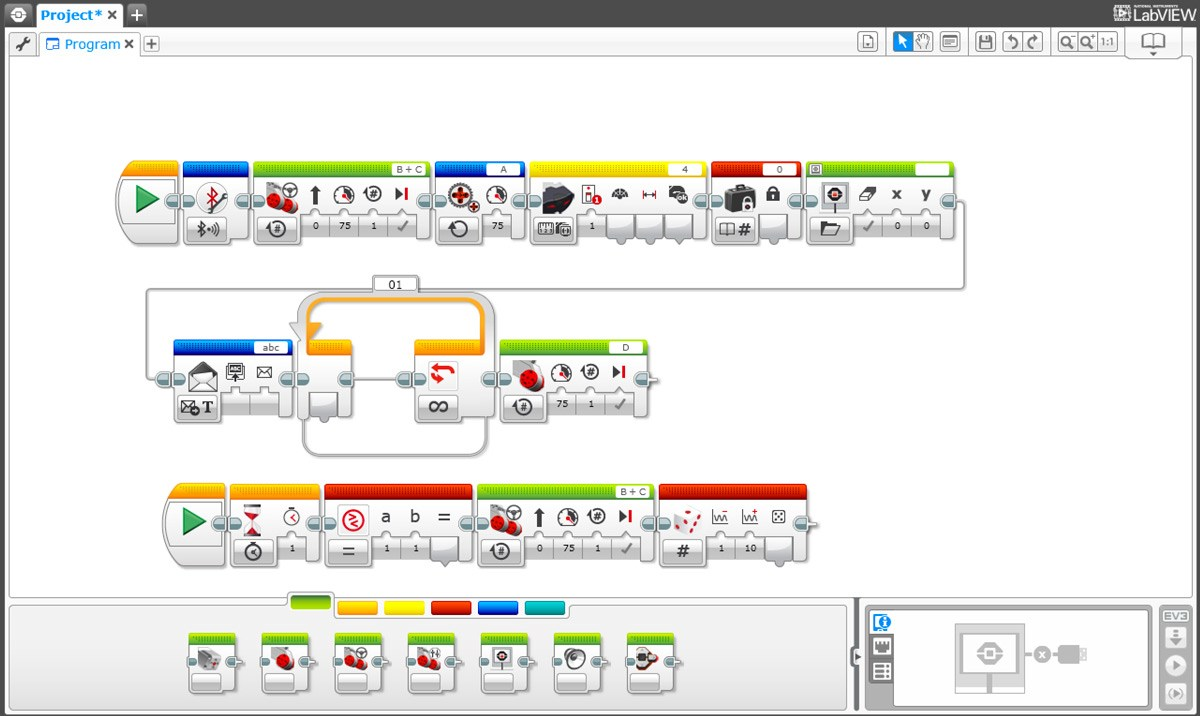
\includegraphics[width=\textwidth]{img/lego2.jpg}
            \caption{Interfaz gráfica de LEGO MINDSTORMS EV3} 
            \label{fig:lego2}
        \end{subfigure}
    \end{figure}

    \item \textit{Kodu}\footnote{\url{https://www.kodugamelab.com}}: lenguaje de programación visual creado por Microsoft para desarrollar videojuegos. Diseñado para ser muy accesible y agradable para cualquier usuario siendo un lenguaje basado en reglas, condiciones y acciones prescindiendo de muchas convecciones de programación como bucles, subrutinas o variables simbólicas. Permite a los más jóvenes a ser creadores de sus propios videojuegos.  
    
    \begin{figure}[H]
        \centering
        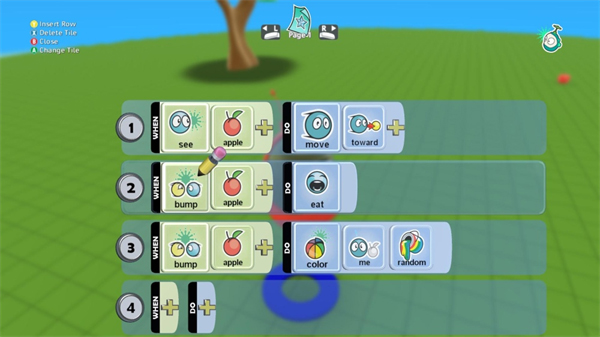
\includegraphics[width=1\textwidth]{img/kodu.jpg}
        \caption{Interfaz gráfica de Kodu} \label{fig:kodu}
    \end{figure}
    
    \item \textit{Snap!\footnote{\url{https://snap.berkeley.edu}}}: basado en \textit{Scratch}, sigue su facilidad para aprender a programar pero su uso se concentra en edades algo más avanzadas. Accesible desde cualquier navegador al estar programado en \textit{JavaScript}.
    
    \begin{figure}[H]
        \centering
        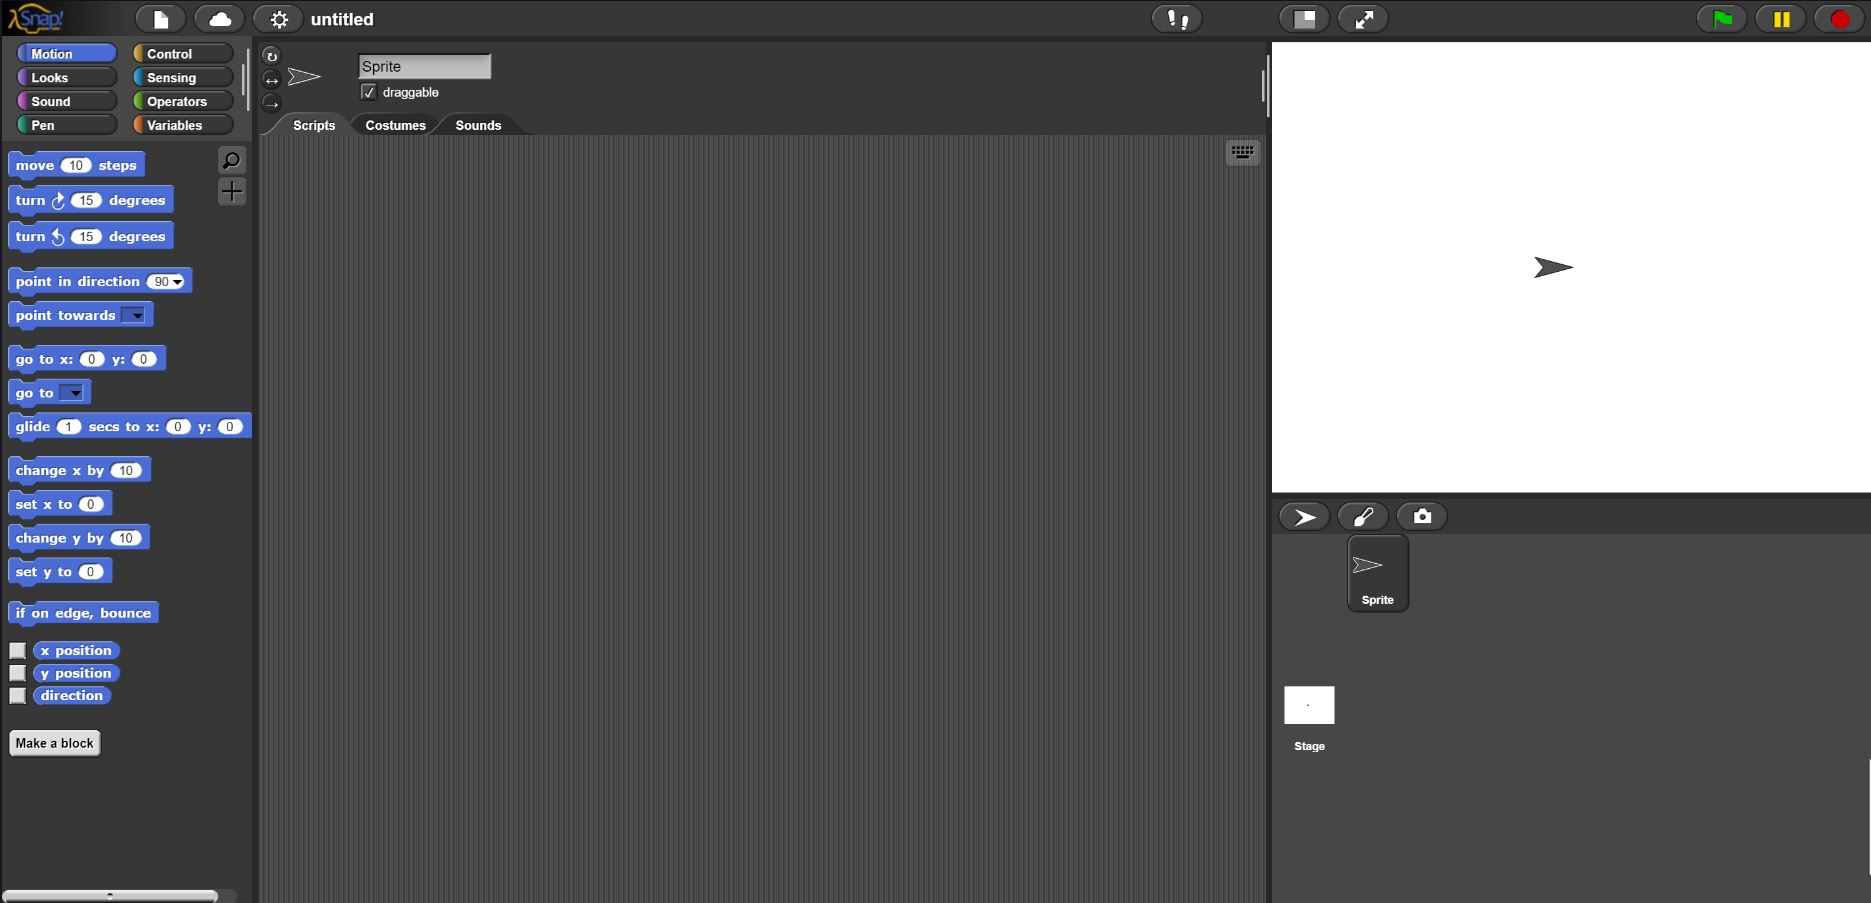
\includegraphics[width=1\textwidth]{img/snap.jpg}
        \caption{Interfaz gráfica de Snap!} \label{fig:snap}
    \end{figure}
\end{itemize}


